\documentclass[
    11pt,
    spanish,
	a4paper
]{article}
\usepackage[utf8]{inputenc}
\usepackage[spanish]{babel}
\usepackage{graphicx}
\usepackage{authoraftertitle}
\usepackage{float}
\usepackage{caption}
\usepackage{verbatim}
\usepackage{listings}
\captionsetup[table]{labelformat=empty}

\def\doctype{Trabajo práctico}
\title{EDU-CIAA}
\author{Gonzalo Nahuel Vaca}

\begin{document}

\makeatletter
\begin{titlepage}
	\begin{center}
		\vspace*{1cm}
		
		\Huge
		\textbf{\doctype}
		\vspace{0.5cm}
    
		\LARGE
		\@title
		\vspace{0.5cm}
    
		\textbf{Procesamiento Digital de Señales (fundamentos)}
		
		\vspace{1.5cm}
		
		\textbf{\@author}

		\vspace{1.5cm}

		
\includegraphics[width=0.8\textwidth]{img/logoFIUBA.pdf}
		
		\vfill
		Maestría en Sistemas Embebidos\\
		Universidad de Buenos Aires\\
		Argentina\\
		\today
	\end{center}
\end{titlepage}
\makeatother
\newpage

\section{Resolución punto 2}

Código Python:

\begin{lstlisting}
from serial import Serial
import numpy as np
import matplotlib.pyplot as plt


if __name__ == "__main__":
  SIZE = 1000
  index = 0
  values = np.arange(SIZE)
  val = 0
  while True:
    with Serial('/dev/ttyACM0', 115200, timeout=1) as usb:
        x = usb.read()
        if(x == b'<'):
          val = int.from_bytes(usb.read(2), byteorder='big')
          if(index < SIZE):
            values[index] = val
            index = index + 1
          else:
            maximo = np.amax(values)
            minimo = np.amin(values)
            rms = np.sqrt(np.mean(values**2))
            print('maximo', maximo, 'minimo', minimo, 'rms', rms)
            index = 0
\end{lstlisting}

Código C:

\begin{lstlisting}
#include "main.h"
#include "arm_math.h"
#include "arm_const_structs.h"

typedef struct
{
	uint32_t wait_time;
	uint32_t systick_limit;
} systick_delay_t;

typedef struct
{
	char head;
	uint16_t val;
} data_frame_t;

static data_frame_t data_frame = {
		.head = '<',
		.val = 0
};

#define MAX_ID 10000

void systick_delay_init(systick_delay_t * delay,
                        uint32_t milliseconds);
void systick_delay(systick_delay_t * delay);

extern UART_HandleTypeDef huart3;
extern ADC_HandleTypeDef hadc1;

void app_launch()
{
	systick_delay_t dsp_delay;
	systick_delay_init(&dsp_delay, 1);
	while(1)
	{

		/* ADC read */
		HAL_ADC_Start(&hadc1);
		HAL_ADC_PollForConversion(&hadc1, HAL_MAX_DELAY);
		data_frame.val = HAL_ADC_GetValue(&hadc1);
		data_frame.head = '<';

		/* UART Transmit */
		HAL_UART_Transmit(&huart3, (uint8_t *)&data_frame,
                      sizeof(data_frame_t), HAL_MAX_DELAY);

		/* Consume time to keep the fs stable */
		systick_delay(&dsp_delay);
	}
}

void systick_delay_init(systick_delay_t * delay,
                        uint32_t milliseconds)
{
	delay->wait_time = milliseconds;
	delay->systick_limit = HAL_GetTick()
                       + delay->wait_time;
}

void systick_delay(systick_delay_t * delay)
{
	while(HAL_GetTick() < delay->systick_limit);
	systick_delay_init(delay, delay->wait_time);
}
\end{lstlisting}

Mediciones en 10 bits:

\begin{lstlisting}
maximo 255 minimo 0 rms 133.4456780866282
maximo 255 minimo 1 rms 132.7910162623963
maximo 255 minimo 0 rms 133.21147473097054
maximo 255 minimo 0 rms 133.96841045559958
maximo 255 minimo 0 rms 132.98777387414228
maximo 255 minimo 0 rms 132.2682350377444
maximo 255 minimo 0 rms 133.78949136610095
maximo 255 minimo 2 rms 133.07224729446784
maximo 255 minimo 0 rms 133.63773793356427
maximo 255 minimo 0 rms 135.09861213202745
maximo 255 minimo 0 rms 134.22736680722005
maximo 255 minimo 0 rms 132.28437171487795
maximo 255 minimo 0 rms 133.7029543428267
maximo 254 minimo 1 rms 132.90886351180646
maximo 255 minimo 0 rms 134.0342195112875
maximo 255 minimo 0 rms 133.7028533726936
maximo 255 minimo 0 rms 132.64832829704264
maximo 255 minimo 0 rms 132.73181231340135
maximo 255 minimo 0 rms 132.97787409941552
maximo 255 minimo 1 rms 132.31173795245832
maximo 255 minimo 0 rms 131.75173243642757
maximo 255 minimo 0 rms 132.91136520252886
maximo 255 minimo 0 rms 133.80505595828583
maximo 255 minimo 0 rms 133.29357448879523
maximo 255 minimo 0 rms 133.01397295021303
maximo 255 minimo 0 rms 132.3346779948476
maximo 255 minimo 1 rms 132.04128899704062
maximo 255 minimo 0 rms 133.09317788677225
maximo 255 minimo 0 rms 133.1260455358004
\end{lstlisting}

Mediciones en 8 bits:

\begin{lstlisting}
maximo 233 minimo 74 rms 162.78772988158536
maximo 233 minimo 74 rms 162.90111724601522
maximo 233 minimo 74 rms 162.7428185819577
maximo 233 minimo 74 rms 162.924654365139
maximo 233 minimo 74 rms 162.9218677771649
maximo 233 minimo 74 rms 162.91097875833907
maximo 233 minimo 74 rms 163.15480072618152
maximo 233 minimo 74 rms 162.55540286314692
maximo 232 minimo 74 rms 163.27862995505566
maximo 233 minimo 74 rms 160.97805129892708
maximo 233 minimo 75 rms 162.93496555374477
maximo 233 minimo 74 rms 163.2358477786053
maximo 233 minimo 74 rms 162.80947761110224
maximo 233 minimo 74 rms 162.93692030967077
maximo 233 minimo 74 rms 162.9120437536771
maximo 233 minimo 74 rms 162.91878344745888
maximo 233 minimo 74 rms 162.6127209046082
maximo 233 minimo 74 rms 162.96469863132936
maximo 233 minimo 74 rms 162.97167545312897
maximo 233 minimo 74 rms 163.13501157017154
maximo 233 minimo 74 rms 163.02364245716018
maximo 233 minimo 74 rms 162.92868071644108
maximo 233 minimo 74 rms 163.17621150155435
maximo 233 minimo 74 rms 163.00040183999548
maximo 233 minimo 74 rms 162.82957962237697
maximo 233 minimo 74 rms 163.07375325293768
maximo 234 minimo 73 rms 162.8507261267201
maximo 233 minimo 73 rms 162.71052516662834
maximo 233 minimo 74 rms 162.86211038789838
maximo 234 minimo 74 rms 162.60057502973353
maximo 233 minimo 74 rms 162.69291010981394
\end{lstlisting}

Se puede apreciar una diferencia producto del error de cuantización.

\begin{figure}[htbp]
	\centering
	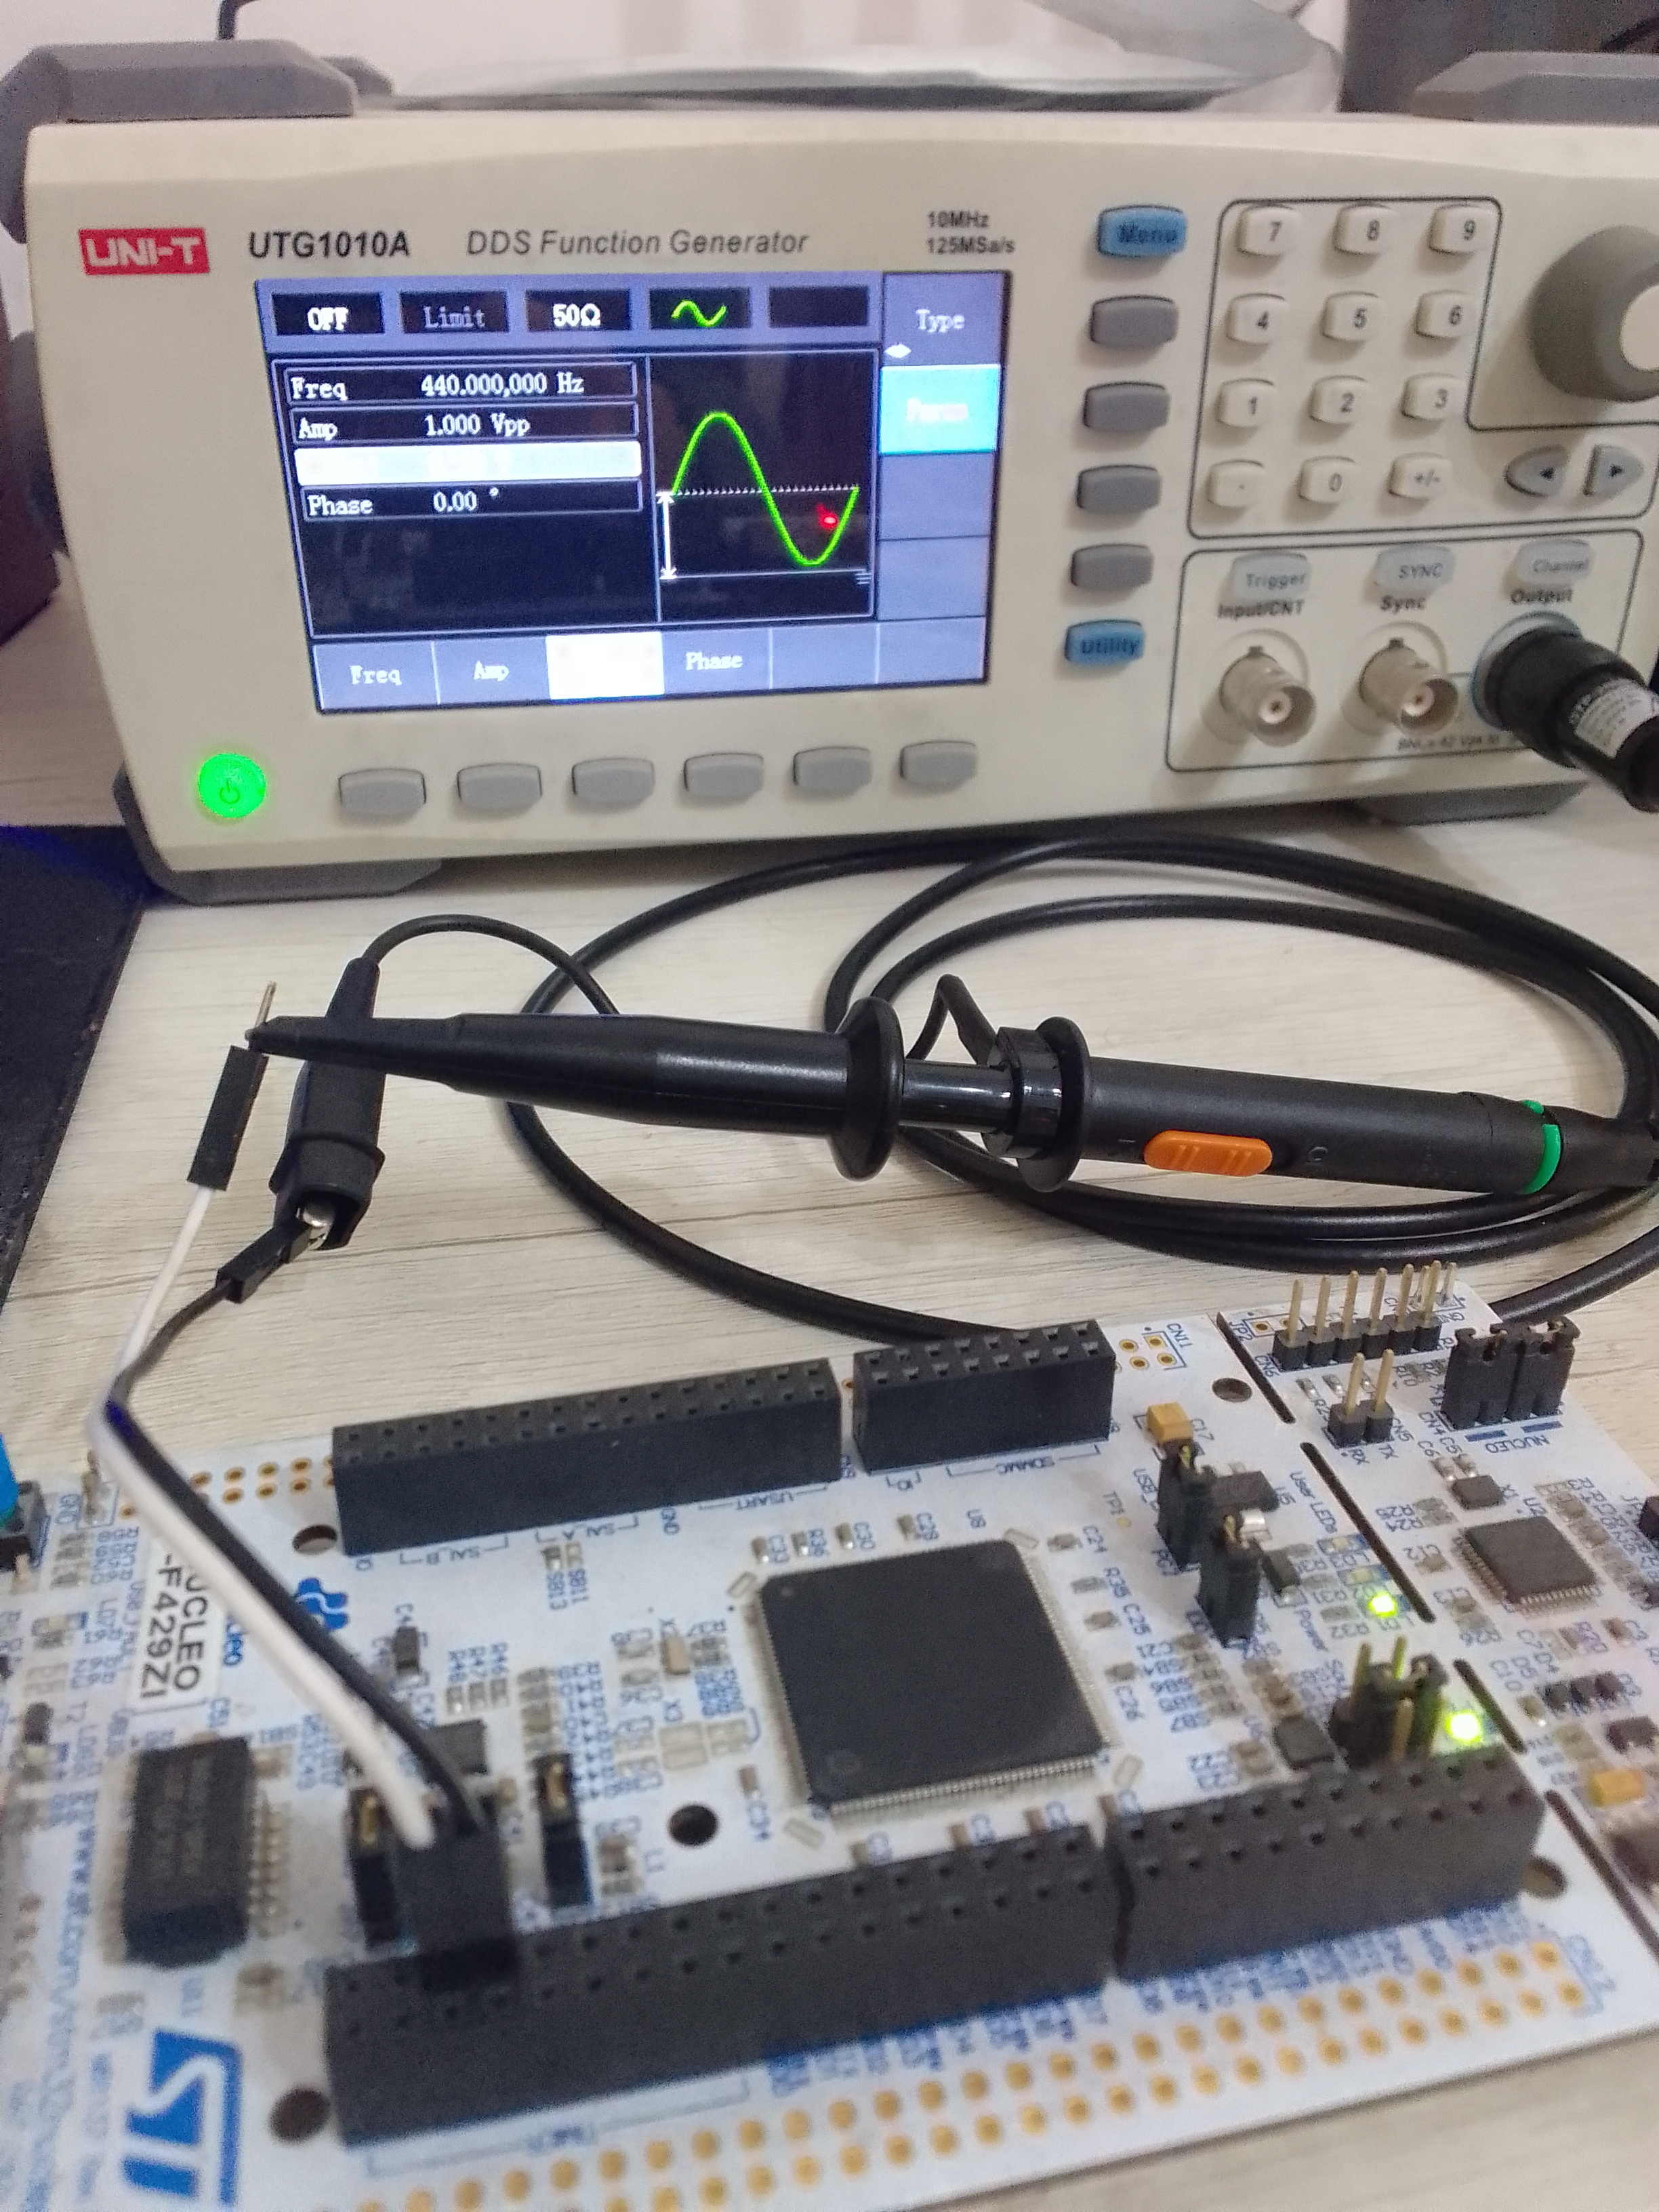
\includegraphics[width=\textwidth]{img/h1.jpg}
	\caption{Fotografía del hardware.}
	\label{fig:h1}
\end{figure}

\begin{figure}[htbp]
	\centering
	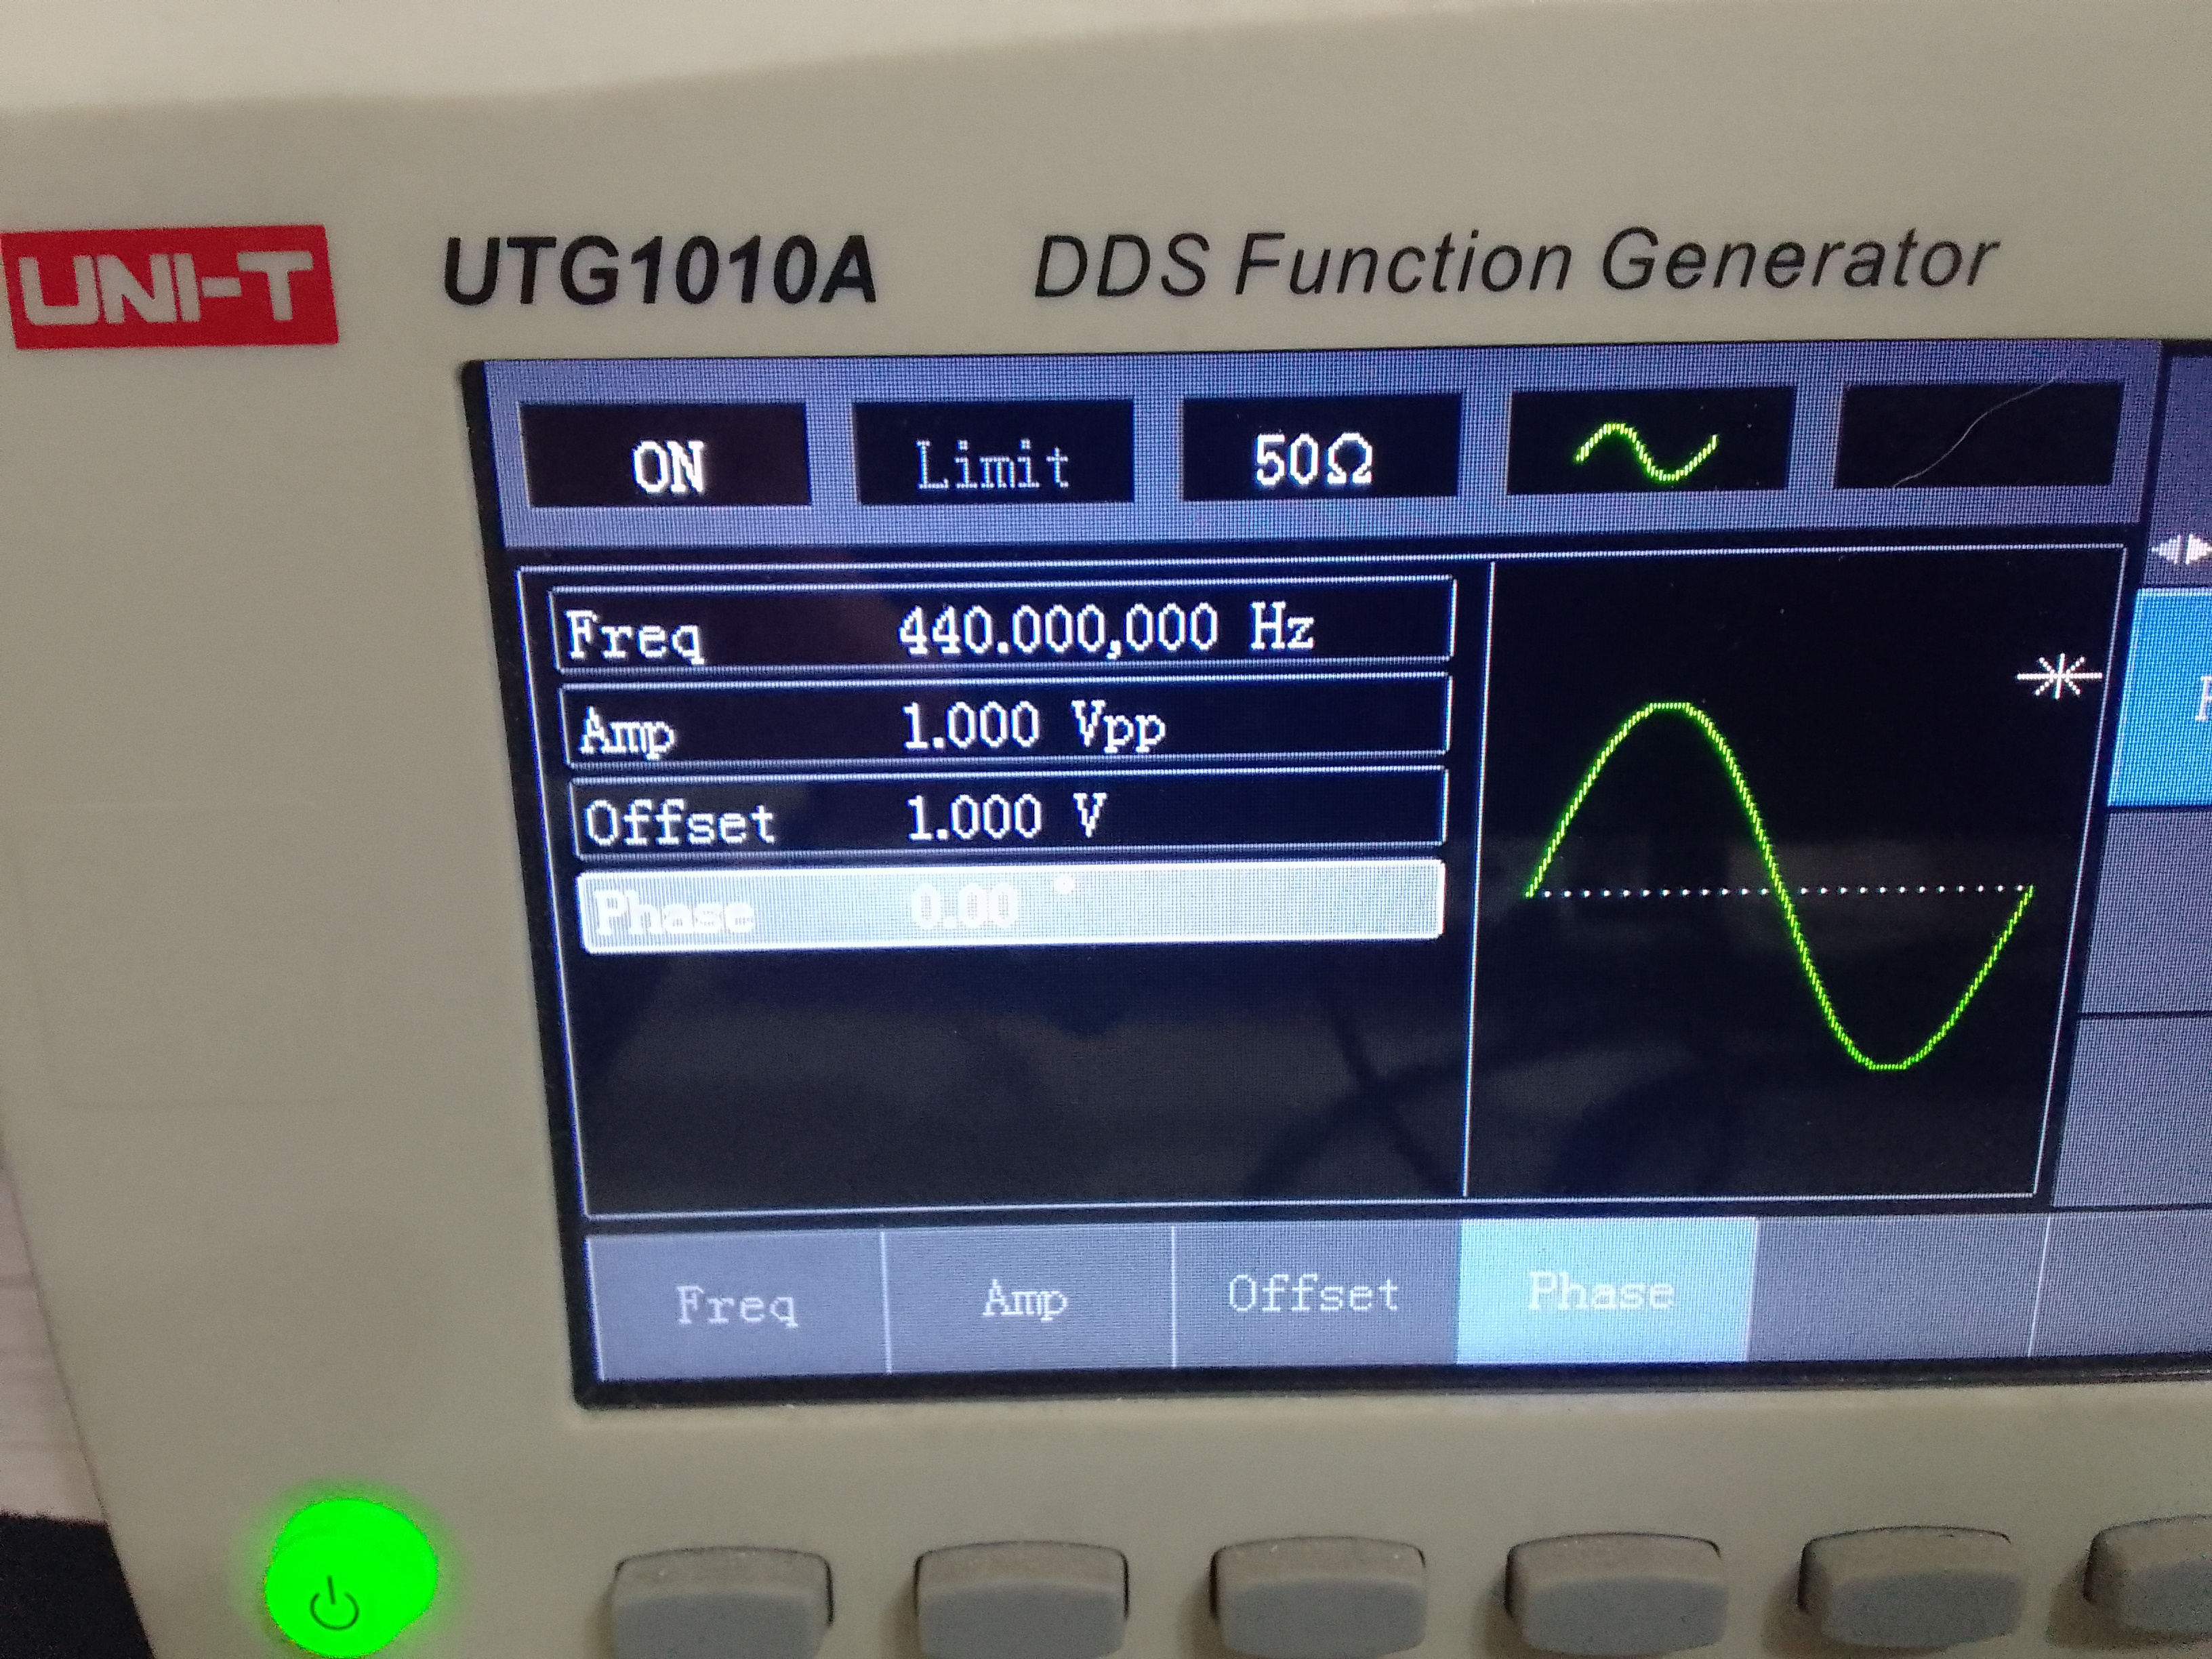
\includegraphics[width=\textwidth]{img/h2.jpg}
	\caption{Detalles de la señal.}
	\label{fig:h2}
\end{figure}

\end{document}
